
\begin{center}
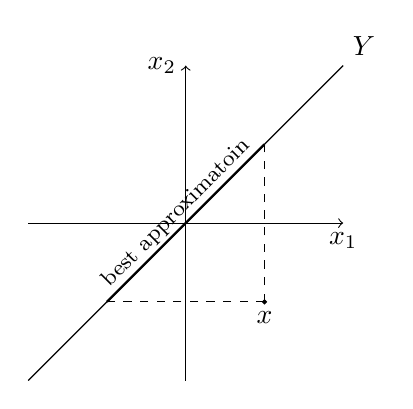
\begin{tikzpicture}
    \draw[->] (0,2) -- (4,2) node [below]  {$x_1$};
    \draw[->] (2,0) -- (2, 4) node [left] {$x_2$};
    \draw (0,0) -- (2,2) node [rotate =45, yshift=5] {
        \footnotesize best approximatoin} -- (4,4) node [above right] {$ Y $};


    \draw[fill] (3,1) circle [radius=0.025];
    \node [below] at (3,1) {$x$};

    \draw[dashed] (3,1) -- (3,3);
    \draw[dashed] (3,1) -- (1,1);
    
    \draw [thick] (3,3) -- (1,1);

\end{tikzpicture}
\end{center}
